\chapter{Vision Module}
\label{cha:vision}

The vision module contains structures and methods for computer vision and contains the following sub-modules:

\begin{description}
% \item[Overlay]~: Module with structures and methods for image overlaying.
\item[Image]~: Module with structures and methods for manipulating several image format~;
\item[Image Mask]~: Module with structures and methods for image mask manipulation.
\item[Image Display]~: Module with structures and methods for image display.
\item[Identification]~: Module with structures and methods for image identification.

\end{description}

%\input{vision/overlay}
\section{Image}
\label{sec:image}

The image module contains structures and methods for manipulating several image formats. 

\subsection{The object {\tt Rox\_Image}}
\label{sse:image_object}

An image object can be declared using the pointer to a \lstinline$Rox_Image_Struct$ structure. 
\begin{lstlisting}
typedef struct Rox_Image_Struct* Rox_Image;
\end{lstlisting}

\subsection{Creating/Deleting a {\tt Rox\_Image}}
\label{sse:image_newdel}

Functions are provided to allocate and deallocate a \lstinline$Rox_Image$ object~:

\begin{lstlisting}
Rox_Error rox_image_new(Rox_Image * image, Rox_Uint cols, Rox_Uint rows);
\end{lstlisting}

The function allocates memory for data depending parameters  `cols' and `rows' which correspond to image size.\\

An image can be created by directly reading a PGM file from disk using the following function:
\begin{lstlisting}
Rox_Error rox_image_new_readpgm (Rox_Image *image, const char *filename);
\end{lstlisting}
The function first allocate memory for the structure with the rows and
cols parameters matching the image file to load. Then it stores the
image data in the image object.

The following function deallocates memory for a \lstinline$Rox_Image$:
\begin{lstlisting}
Rox_Error rox_image_del(Rox_Image * image);
\end{lstlisting}
 It is necessary to call this function when the object is not used anymore.


\subsection{Main functions related to {\tt Rox\_Image}}
\label{sse:image_functs}

Once the object \lstinline$Rox_Image$ has been allocated, it is possible to get information from \lstinline$Rox_Image$.

\begin{description}
% \item [rox\_image\_get\_data]~: Get the pointer of the first pixel intensity values.
  \item [rox\_image\_get\_rows]~: Get the image rows.
  \item [rox\_image\_get\_cols]~: Get the image columns.
\end{description}

An image can be read from a PGM file if the size is compatible.
Typically, we use a \lstinline$rox_image_new_readpgm$ function to
read the first image of a sequence and allocate correctly the
corresponding structure. Then, assuming that all images of a sequence
have the same dimensions, we can re-use the same structure for the
next images, using the \lstinline$rox_image_readpgm$ function. Thus,
the structure is safely allocated while loading the reference image
and the other images are read previously to perform the tracking.
Currently, the only supported format in the library is raw PGM
(Portable Gray Map) \footnote{{http://netpbm.sourceforge.net/doc/pgm.html}}:
\begin{lstlisting}
Rox_Error rox_image_readpgm (Rox_Image image, const char *filename);
\end{lstlisting}
The function returns an error if the dimensions of the image file do not match the dimesions of the allocated image.

External libraries can be easily used to read images from files. Then,
\rox{} allows to input several image formats. The list of
available image formats is given in the enumeration
\lstinline$Rox_Image_Format_Enum$ (see the Programmer Manual for a
complete list):

\begin{lstlisting}
enum Rox_Image_Format_Enum{
     Rox_Image_Format_Grays,
     Rox_Image_Format_YUV422,
     Rox_Image_Format_Color_RGBA,
     Rox_Image_Format_Color_BGRA,
     Rox_Image_Format_Color_ARGB,
     Rox_Image_Format_Color_BGR,
     Rox_Image_Format_Color_RGB
};
\end{lstlisting}

The image data can be set using the following function:
\begin{lstlisting}
Rox_Error rox_image_set_data (Rox_Image image, Rox_Uchar *data, Rox_Uint bytesPerRow, enum Rox_Image_Format format);
\end{lstlisting}
This function transforms an external image buffer to the rox internal
format and store this information inside the Rox\_Image object.  The
input image format shall be a 3 or 4 channel interleaved image
containing Red, Blue and Green channels.  Only one of these channels
(specified by the channel parameter) will be used while converting to
rox internal format.  User needs to specify the exact format of the
input buffer (e.g. RGB, BGR, RGBA, etc.) as it is impossible to guess
it automatically, as well as how many bytes are used per row in the
input image.

Finally, in order to know if an image suitable for identification and odometry computation, the following functions allows to get a quality score.

The first function is fast but do not provide precise information: 
\begin{lstlisting}
Rox_Error rox_image_get_quality_score (Rox_Real *score, Rox_Image image);
\end{lstlisting}

The second function is slower but provides precise information on the quality of an image:
\begin{lstlisting}
Rox_Error rox_image_get_quality_score_precise (Rox_Real *score, Rox_Image image);
\end{lstlisting}

\section{Image mask}
\label{sec:imask}

\subsection{The object {\tt Rox\_Imask}}
\label{sse:imask_object}

The image structures of {\bf \rox} can be coupled with an image mask structure \lstinline$Rox_Imask_Structure$ that contains a mask. % represented as a byte (unsigned char) tab. 

A mask can be declared using the pointer \lstinline$Rox_Imask$ to a \lstinline$Rox_Imask_Structure$:
 
\begin{lstlisting}
typedef struct Rox_Imask_Struct* Rox_Imask;
\end{lstlisting}

\subsection{Creating/Deleting a {\tt Rox\_Imask}}
\label{sse:creating_imask}
Functions are provided to allocate and deallocate a \lstinline$Rox_Imask$ object~:

\begin{lstlisting}
Rox_Error rox_imask_new(Rox_Imask * imask, Rox_Uint cols, Rox_Uint rows);
\end{lstlisting}
The \lstinline$rox_imask_new$ function allocates memory for a mask object. In this case, the size of allocated memory depends on parameters `cols' and `rows'.\\ 

The \lstinline$rox_imask_del$ function deallocates memory for a mask object. 
\begin{lstlisting}
Rox_Error rox_imask_del(Rox_Imask * M);
\end{lstlisting}
It is necessary to call this function when the structure is not used anymore.

\subsection{Main functions related to {\tt Rox\_Imask}}
\label{sse:imask_methods}

To each pixel of an image corresponds a mask information. If a mask byte is set to 0 (zero), then the corresponding pixel shall be ignored. If a mask byte is set to $\sim$0 (bitwise complement to zero), then the corresponding pixel shall be considered.  By default, an image mask is fully set to  $\sim$0 (bitwise complement to zero). \\

The user can easily define his own mask for a given image. The main
application in the tracking algorithm is to define a non-rectangular
reference region. For example, it is possible to define a circle where
all mask bytes inside this circle are set to  $\sim$0 (bitwise complement to zero) and all
others to 0 (zero). Thus the region to track is not a rectangle but a
circle, even if the image structure represents a rectangular region of
interest.\\

The user can create his own functions to set the image mask as he
wants. The only thing to do is to set to 0 the mask bytes
corresponding to ignored pixels and to  $\sim$0 (bitwise complement to zero) all the others.\\

A function is available to fill a mask object with user defined data~:

\begin{lstlisting}
void rox_imask_set_user(Rox_Imask imask, const Rox_Uchar* data);
\end{lstlisting}

\noindent The `imask' parameter is a \lstinline$Rox_Imask$ structure already allocated with \lstinline$rox_imask_new$. 
The second parameter contains the mask values defined by the user. \\

\noindent The following functions are provided to create basic masks:
\begin{description}
  \item[rox\_imask\_set\_zero]~: Sets the mask values to zero.
  \item[rox\_imask\_set\_one]~: Sets the mask values to one.
  \item[rox\_imask\_set\_ellipse]~: Sets a mask with elliptic shape.
%  \item[rox\_imask\_set\_polygon]~: Sets the image mask inside a polygon .
\end{description}

\noindent Example of mask objects settings~:
\begin{lstlisting}
{
  // Create and allocate Rox_Imask structures
  Rox_Uint size = 64; // The mask will be square
  Rox_Imask Ellipse = rox_imask_new(size, size);
  Rox_Imask User_defined = rox_imask_new(size, size);
  Rox_Imask Polygon = rox_imask_new(size, size);
  Rox_Imask Combination = rox_imask_new(size, size);
 
  // Data for the mask defined by the user
  Rox_Uchar Data[size * size];

  // Initialize Data
  for(int i = 0; i<size; i++)
  {
    for(int j = 0; j<size; j++)
	Data[i+j*size] = ~0;
  }

  for(int i = size/2; i<size; i++)
  {
    for(int j = 0; j<size/2; j++)
	Data[i+j*size] = 0;
  }

  for(int i = 0; i<size/2; i++)
  {
    for(j = size/2; j<size; j++)
	Data[i+j*size] = 0;
  }
   
  //Initialize points for polygon data (In this example, it is a triangle)
  const Rox_Uint points [6] = { 4, 3, 50, 32, 14, 57}; 

  // Set Masks
  rox_imask_set_ellipse(Ellipse);
  rox_imask_set_user(User_defined, Data);
  rox_imask_set_polygon(Polygon, points, 3);
  rox_imask_set_and(Combination, Polygon, User_defined);

  // Save masks
  rox_imask_savepgm("Ellipse.pgm", Ellipse);
  rox_imask_savepgm("User.pgm", User_defined);  
  rox_imask_savepgm("Combination.pgm", Combination);
  rox_imask_savepgm("Polygon.pgm", Polygon);

  // Free Memory
  rox_imask_del(User_defined);
  rox_imask_del(Ellipse);
  rox_imask_del(Polygon);
  rox_imask_del(Combination);
}
\end{lstlisting}

In the figure \ref{fig:mask}, you can see the example results.
In order of appearance, the masks are: Ellipse, User, User-Ellipse combination and Polygon. 
\begin{figure}[htbp] 
\begin{center}
 
\includegraphics[width=0.24\textwidth]{vision/figures/Ellipse}  
 
\includegraphics[width=0.24\textwidth]{vision/figures/User}  
 
\includegraphics[width=0.24\textwidth]{vision/figures/And}
 
\includegraphics[width=0.24\textwidth]{vision/figures/Polygon}  \\ 
 \caption{Examples of setting masks.}
\label{fig:mask}
\end{center}
\end{figure} 

\section{Image Display}
\label{sec:idisp}

The image display module contains structures and methods for displaing results on images and saving on disk. 

\subsection{The object {\tt Rox\_Image\_Display}}
\label{sse:idisp_object}

An image display object can be declared using the pointer to a \lstinline$Rox_Image_Display_Struct$ structure. 
\begin{lstlisting}
typedef struct Rox_Image_Display_Struct* Rox_Image_Display;
\end{lstlisting}

\subsection{Creating/Deleting a {\tt Rox\_Image\_Display}}
\label{sse:idisp_newdel}

Functions are provided to allocate and deallocate a \lstinline$Rox_Image_Display$ object~:

\begin{lstlisting}
Rox_Error rox_image_display_new (Rox_Image_Display *image, Rox_Uint cols, Rox_Uint rows);
\end{lstlisting}

The function allocates memory for data depending parameters  `cols' and `rows' which correspond to image size.\\

\begin{lstlisting}
Rox_Error rox_image_display_del (Rox_Image_Display *image);
\end{lstlisting}

The function deallocates memory for a \lstinline$Rox_Image_Display$ object. It is necessary to call this function when the
structure is not used anymore.

\subsection{Main functions related to {\tt Rox\_Image\_Display}}
\label{sse:idisp_functs}

An image can be read from a PGM or PPM file if the size is compatible using the following functions:

\begin{lstlisting}
Rox_Error rox_image_display_readpgm (Rox_Image_Display image, const char *filename);
\end{lstlisting}

\begin{lstlisting}
Rox_Error rox_image_display_readppm (Rox_Image_Display image, const char *filename);
\end{lstlisting}

After drawing the results, the image can be saved on disk using the following functions:

\begin{lstlisting}
Rox_Error rox_image_display_savepgm (const char *filename, Rox_Image_Display image);
\end{lstlisting}

\begin{lstlisting}
Rox_Error rox_image_display_saveppm (const char *filename, Rox_Image_Display image);
\end{lstlisting}

The results of odometry computation can be drwan using the following functions:
\begin{lstlisting}
Rox_Error rox_image_display_draw_projection_model_single_plane (Rox_Image_Display image, Rox_Matrix calib, Rox_MatSE3 pose, Rox_Model_Single_Plane model, Rox_Uint color);
\end{lstlisting}

\begin{lstlisting}
Rox_Error rox_image_display_draw_projection_model_multi_plane (Rox_Image_Display image, Rox_Matrix calib, Rox_MatSE3 pose, Rox_Model_Multi_Plane model, Rox_Uint color);
\end{lstlisting}

\section{Identification}
\label{sec:ident}

The identification module contains structures and methods for the identification of model images and contains the following sub-modules:

\begin{description}

\item[Photoframe identification]~: Module with structures and methods for texture identification using a photoframe around the model image.
\item[Texture identification]~: Module with structures and methods for texture identification. This module allows the user to define textured model images. The identification at run-time is generally slower than the database identification but can be accelerated using a photoframe around the model image.
\item[Database identification]~: Module with structures and methods for model identification in a database.The database identification module needs the generation of a database from an image model. This offline generation step is time consuming but can be performed once and for all. At runtime, the database identification is faster than the texture identification since many computations have already been done offline.
\end{description}

\subsection{Photoframe identification}
\label{sse:ident_photoframe}

\noindent The photoframe identification module performs the identification of textured model images with a black frame around the texture as shown in Figure~\ref{fig:ident_photoframe}. 

\begin{figure}[H]
\centering
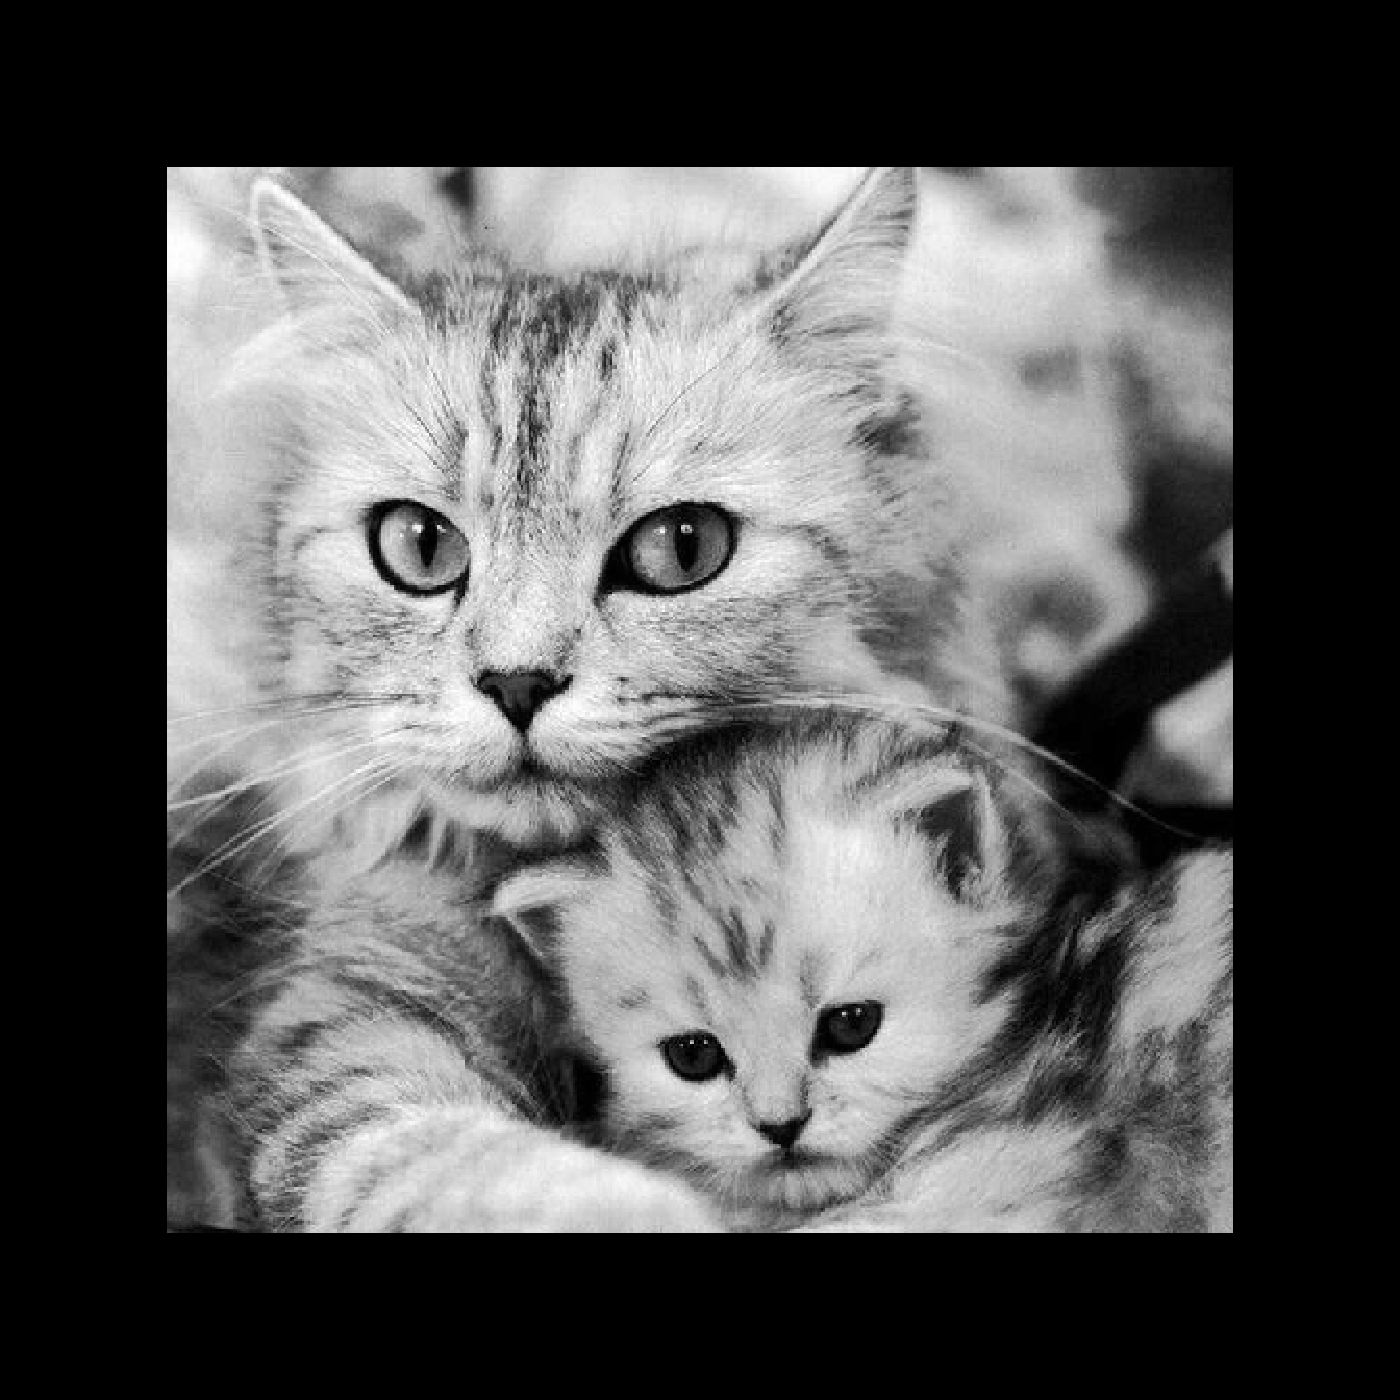
\includegraphics[width=0.45\textwidth]{vision/figures/ident_photoframe} 
\caption{Examples of model that can be identified with the photoframe identification module.}
\label{fig:ident_photoframe}
\end{figure}

The photoframe image model identification is faster than the
identification of phototexture image model since the identification
take benefit of the detection of the black frame around the texture.
On the other hand, the black frame shall be fully visible in the image.

\subsubsection{The {\tt Rox\_Ident\_Photoframe\_SE3} object}
\label{sss:ident_photoframe_object}
A \lstinline$Rox_Ident_Photoframe_SE3$ object is a pointer to the opaque structure \lstinline$Rox_Ident_Photoframe_SE3_Struct$: 

\begin{lstlisting}
typedef struct Rox_Ident_Photoframe_SE3_Struct * Rox_Ident_Photoframe_SE3
\end{lstlisting}

\subsubsection{Creating/Deleting a {\tt Rox\_Ident\_Photoframe\_SE3}}
\label{sss:ident_photoframe_newdel}
~\\

\noindent The rox\_ident\_photoframe object shall be created before any call to other functions using it :

\begin{lstlisting}
Rox_Error rox_ident_photoframe_new(Rox_Ident_Photoframe * ident_photoframe) 
\end{lstlisting}

\noindent This function creates a new empty database object.

\begin{lstlisting}
Rox_Error rox_ident_photoframe_del(Rox_Ident_Photoframe * ident_photoframe)
\end{lstlisting}


\subsubsection{Main functions related to {\tt Rox\_Ident\_Photoframe\_SE3}}
\label{sss:ident_photoframe_functions}
~\\

\noindent A photoframe is a planar object specifically designed to be identified
when filmed with a camera. It is a composition of an image template, a
thick black border and a white background outside of the border.
Figure 1 explains the common scheme of a photoframe.  The image inside
the black borders is the \emph{template}. This template is the object
to identify, and which will be used to track the object after
detection if needed. This template size is
$\left[image \; rows, image \; cols\right]$.  Values iheight and iwidth shall be
equal to 128 pixels.

\begin{figure}[h]
\centering{}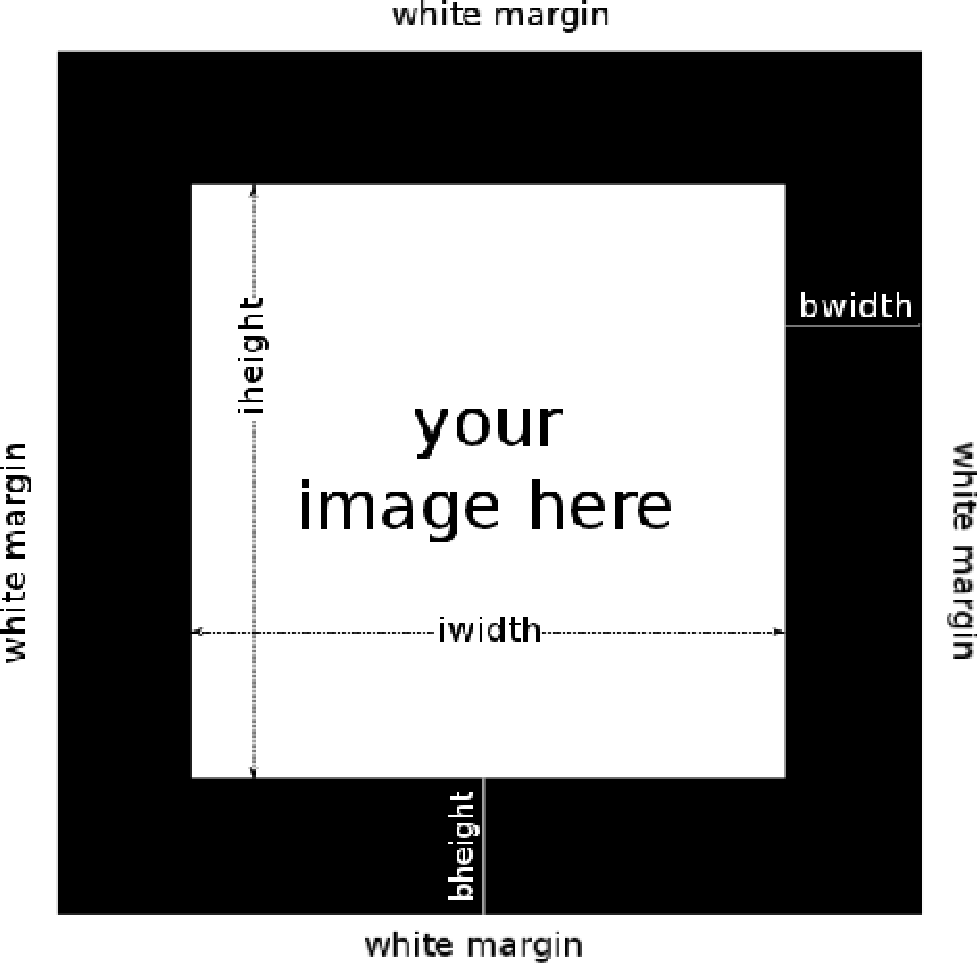
\includegraphics[width=0.6\columnwidth]{vision/figures/fake}
\caption{A common photoframe scheme}
\end{figure}

\noindent The border size $\left[border \; rows, border \;
  cols\right]$ is choosed optimally to be visible in a large set of
viewpoints while not being too large (i.e. not wasting image space).
The following calculus is done to compute border size :

\begin{itemize}
\item border rows = $\frac{80}{512}$ image rows
\item border cols = $\frac{80}{512}$ image cols
\end{itemize}

\noindent Be sure to respect those sizes when creating your photoframe or the
identification performance will be severely degraded.\\

\noindent To create a photoframe, choose a template image which is compatible
with \rox{} (non uniform, with enough texture). Store this template in
a PGM image file. With an image editing software (E.g. : photoshop,
gimp) draw the borders in black color (See figure 1). Print this image
on a white paper sheet. Because of printers approximation, it is not
possible to know what will be the exact size (in meters) of this
print.  Take a ruler to measure the width and height of the image
template \emph{inside} the black borders. These real sizes are only
needed if used to compute odometry after identification. Repeat this
operation for each photoframe you need.\\

\noindent The user can go through the following workflow:

\begin{enumerate}
\item An identification structure is created (see section~\ref{sss:ident_photoframe_newdel}).
\item Template images are added to the identification module using the following function:

\begin{lstlisting}
Rox_Error 	rox_ident_photoframe_se3_addframe (Rox_Ident_PhotoFrame_SE3 obj, Rox_Image model, Rox_Real width_meter, Rox_Real height_meter, Rox_Uint border_width);
\end{lstlisting}

\noindent Adds a new template to a photoframe identification
structure. Shall be called before identification. First parameter is a
pointer created with rox\_ident\_new, second parameter is the template
image to add (without black borders) with a size of 128x128 pixels.
Please note that one photoframe will be identified only once in one
image. If several instances of the same photoframe are in the
processed image, only the first found will be considered. Note that
the identifier of the added photoframe will be the number of times
this function has already been called.

\item The user grabs an image from a stream (e.g. a camera) and gives it
  to photoframe identification. The identification is done and the
  number of identified templates are stored in the \lstinline $Rox_Ident_PhotoFrame_SE3$ object:

\begin{lstlisting}
Rox_Error rox_ident_photoframe_se3_make (Rox_Ident_PhotoFrame_SE3 obj, Rox_Camera camera);
\end{lstlisting}

\noindent Using the ident structure created with rox\_ident\_new and filled
with templates using rox\_ident\_add\_photoframe, tries to detect
photoframes in the given image. This image may be given by a camera
for example. Returns the number of identified photoframes in the current
image.

\item For each template, the user can check if it has been identified using the following function:

\begin{lstlisting}
Rox_Error rox_ident_photoframe_se3_getresult (Rox_Uint *is_identified, Rox_MatSE3 pose, Rox_Ident_PhotoFrame_SE3 obj, Rox_Uint id);
\end{lstlisting}

\noindent Used after a call to rox\_ident\_photoframe. Checks if a given photoframe
(using its id) has been detected or not. ident is a
pointer to a photoframe identification structure created with rox\_ident\_new.
photoframe\_id is a number between 0 and the number of added frames.
Returns Rox\_True if the specific photoframe is detected, Rox\_False
otherwise.

% \item If the template is identified, a function returns a 2D transformation which
% measures how the template is ``seen'' in the current grabbed image.

% \begin{lstlisting}
% Rox_MatSL3 rox_ident_photoframe_get_matsl3(Rox_Ident ident, Rox_Uint id);
% \end{lstlisting}

\noindent Used after a call to rox\_ident\_photoframe and rox\_ident\_get\_identified.
If a photoframe with id has been identified, returns the 2D
transformation which represents the template image (without the borders)
in the current image. 2D transformation is not defined (and may contain
random value) if the marker is not identified.\\

\item Once not used anymore, the identification structure shall
be deleted (see section~\ref{sss:ident_photoframe_newdel}).
\end{enumerate}

\subsection{Texture identification}
\label{sse:ident_texture}

\noindent The texture identification module performs the identification of textured model images as shown in Figure~\ref{fig:ident_texture}. 

\begin{figure}[H]
\centering
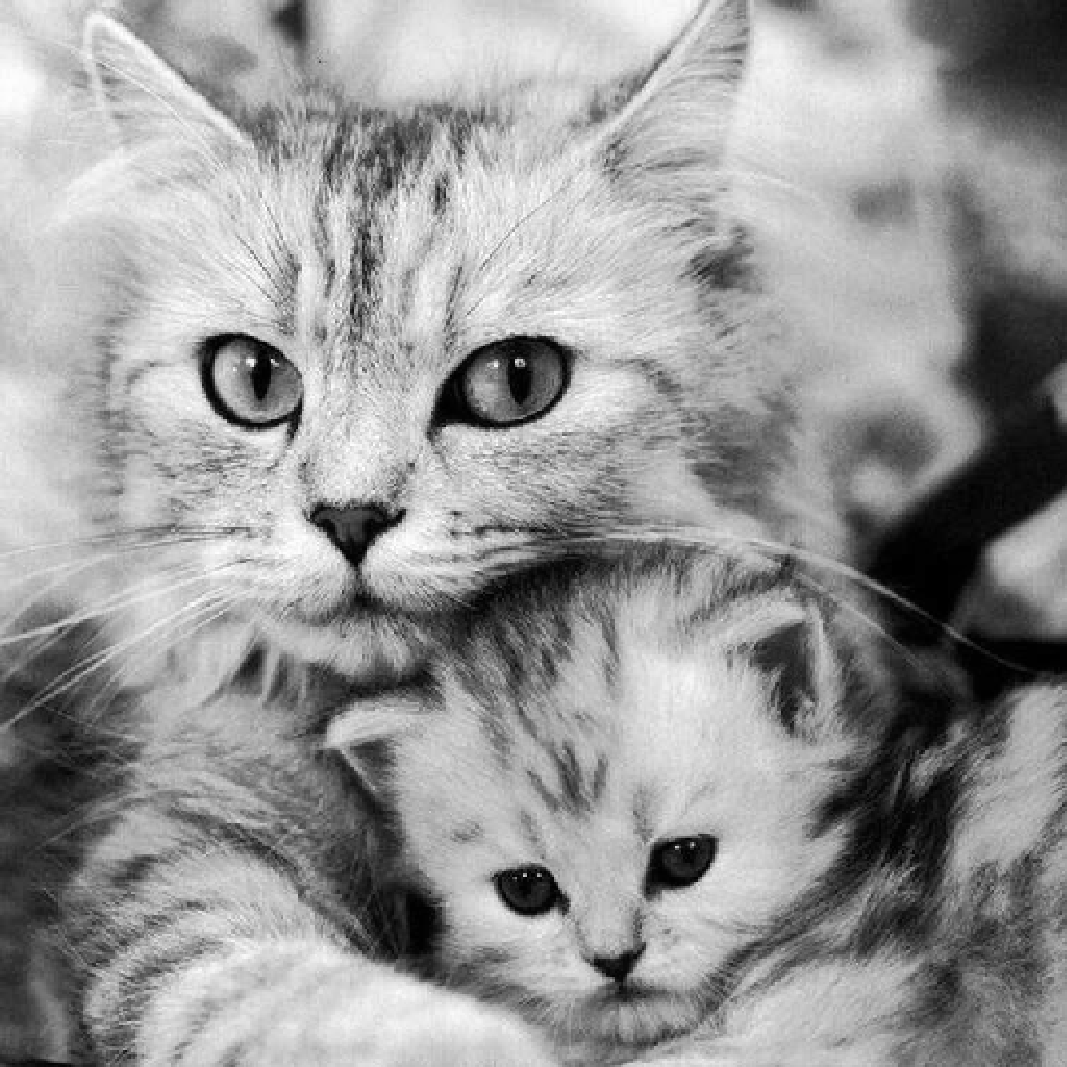
\includegraphics[width=0.45\textwidth]{vision/figures/ident_phototexture} 
\caption{Example of image model that can be identified with the texture identification module.}
\label{fig:ident_texture}
\end{figure}

\subsubsection{The {\tt Rox\_Ident\_Texture\_SE3} object}
\label{sss:ident_texture_object}
A \lstinline$Rox_Ident_Texture_SE3$ object is a pointer to the opaque structure \lstinline$Rox_Ident_Texture_SE3_Struct$: 

\begin{lstlisting}
typedef struct Rox_Ident_Texture_SE3_Struct * Rox_Ident_Texture_SE3
\end{lstlisting}


\subsubsection{Creating/Deleting a {\tt Rox\_Ident\_Texture\_SE3}}
\label{sss:ident_texture_newdel}

\noindent Functions are provided to allocate and deallocate a \lstinline$Rox_Ident_Texture_SE3$ object~:

\begin{lstlisting}
Rox_Error rox_ident_texture_se3_new (Rox_Ident_Texture_SE3 *ident_texture);
\end{lstlisting}

\noindent The function creates a new identification structure. Shall be called before
any other function of this module. Returns a pointer to the Rox\_Ident\_Texture object. \\

\begin{lstlisting}
Rox_Error 	rox_ident_texture_se3_del (Rox_Ident_Texture_SE3 *ident_texture); 
\end{lstlisting}

\noindent Deletes an identification structure. First parameter is a pointer
created with rox\_ident\_texture\_new. Shall be called to free up memory when
user does not need identification anymore.

\subsubsection{Main functions related to {\tt Rox\_Ident\_Texture\_SE3}}
\label{sss:ident_texture_functions}
~\\

A model to be identified can be set using the following function:
\begin{lstlisting}
Rox_Error rox_ident_texture_se3_set_model (Rox_Ident_Texture_SE3 ident_texture, Rox_Model_Single_Plane model); 
\end{lstlisting}
A function is available to identify a given model in a camera object: 
The second function input the camera containing the current image in which to identify the texture:
\begin{lstlisting}
Rox_Error rox_ident_texture_se3_make (Rox_MatSE3 pose, Rox_Ident_Texture_SE3 ident_texture, Rox_Camera camera);
\end{lstlisting}

% If identification is successfull, the resulting homography matrix locating the serched texture in the image can be obtained with the following function: 
% \begin{lstlisting}
% Rox_Bool rox_ident_texture_get_matsl3_copy(Rox_MatSL3 H, Rox_Ident_Texture ident_texture)
% \end{lstlisting}

%\begin{lstlisting}
%Rox_MatSL3 rox_ident_texture_get_matsl3(Rox_Ident_Texture ident_texture) 	
%\end{lstlisting}

\subsection{Database identification}
\label{sse:database}

The computation of visual information (e.g. keypoints features) needed
for image identification can be done offline and stored in a database.
For each image model we would like to identify in the current image, a
specific database item is created. Several items can also mixed
together to allow the identification of multiple images.

Figure~\ref{fig:ident_database} illustrates the structure of the database identification module:

\begin{figure}[H]
\centering
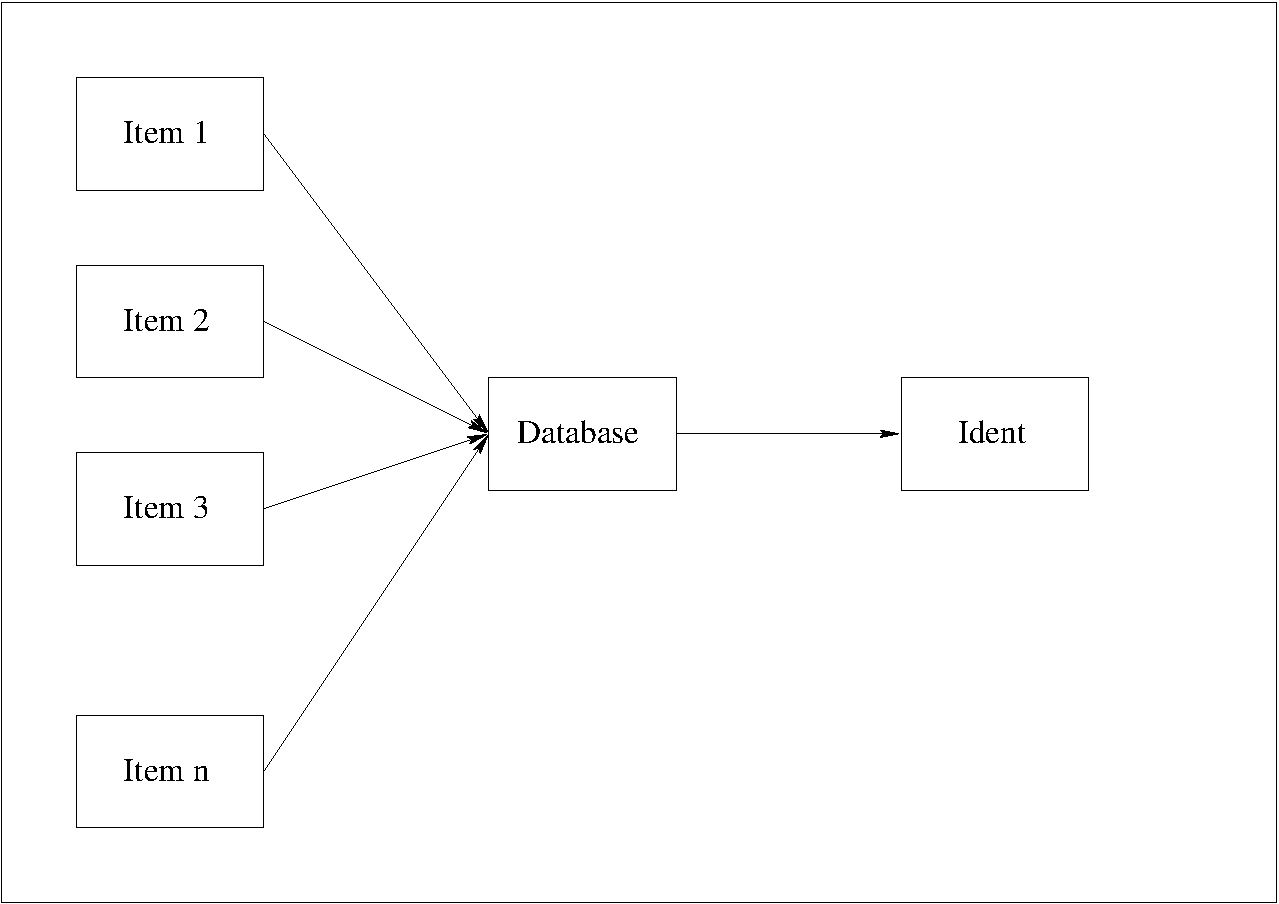
\includegraphics[width=0.75\textwidth]{vision/figures/ident_database} 
\caption{Structure of the database identification module.}
\label{fig:ident_database}
\end{figure}

\subsubsection{The {\tt Rox\_Ident\_Database\_SE3} object}
A \lstinline$Rox_Ident_Database_SE3$ object is a pointer to the opaque structure \lstinline$Rox_Ident_Database_SE3_Struct$: 

\begin{lstlisting}
typedef struct Rox_Ident_Database_SE3_Struct * Rox_Ident_Database_SE3
\end{lstlisting}

\subsubsection{Creating/Deleting a {\tt Rox\_Ident\_Database\_SE3}}

\noindent One database item is associated to one template. A Rox\_Ident\_Database may be considered as a collection of such database items. The database identification module is able to identify several templates simultaneously. Current library is optimized to run on up to 150 simultaneous templates. User can ask the module to detect all possible templates in the same current image or to detect only the most visible template (among the templates in the database). Speed degrades with the number of templates to track simultaneously and quality degrades with the number of templates in the database. It is possible to create several Rox\_Ident\_Database objects in the same program.\\

\noindent The rox\_ident\_database object shall be created before any call to other functions using it :

\begin{lstlisting}
Rox_Error rox_ident_database_se3_new (Rox_Ident_Database_SE3 *ident, Rox_Uint max_templates_simultaneous);
\end{lstlisting}

\noindent This function creates a new empty database object.

\begin{lstlisting}
Rox_Error rox_ident_database_se3_del (Rox_Ident_Database_SE3 *ident);
\end{lstlisting}

This function deletes the object. Shall be called when you do not need this database object anymore.

\subsubsection{Main functions related to {\tt Rox\_Ident\_Database\_SE3}}

% \begin{lstlisting}
% Rox_Bool rox_ident_database_add_template(Rox_Ident_Database
% obj, Rox_Char * pathtodb, Rox_Uint template_height, Rox_Uint template_width)
% \end{lstlisting}

% \noindent This function adds a template database file to the Rox\_Ident\_Database object. Please take care not to add several times the same database file. Template dimensions (template\_height and template\_width) are the dimensions of
% the reduced image to be used for further tracking process. Each time you add a
% template, an internal counter is incremented. The value of this counter is used
% as a unique ID for this template. Thus the template ID is a number between
% 0 and N-1 (N being the number of added templates).

\noindent The following function shall be called to enable
identification and prepare internal structures for optimized
execution:
\begin{lstlisting}
Rox_Error rox_ident_database_se3_set_database (Rox_Ident_Database_SE3 ident, Rox_Database db);
\end{lstlisting}

\noindent The following function execute identification process on the
image contained in the camera object. Uses all the templates added and
compiled before the call to this function. Once a template is found,
an internal flag is set and it will be ignored in further calls to
rox\_ident\_database\_process.
\begin{lstlisting}
Rox_Error rox_ident_database_se3_make (Rox_Ident_Database_SE3 ident, Rox_Camera camera);
\end{lstlisting}

\noindent To get the identification result for a given template ID use the following function: 

\begin{lstlisting}
Rox_Error rox_ident_database_se3_getresult (Rox_Uint *is_identified, Rox_MatSE3 pose, Rox_Ident_Database_SE3 ident, Rox_Uint id); 
\end{lstlisting}

\subsubsection{Creation of database items}

\noindent First, retrieve an image of your template without any perspective distortion. The biggest the image is, the better the detection will perform after database creation. However, if the image is too big the database file will be large and long to create. Ideally, the template size should be close to the image that will be viewed by the camera. The template image shall not contain large textureless regions and shall contain visual information everywhere. Please keep both files in a directory as they will be necessary for identification process.

The programmer can create its own database items by using the following function:
\begin{lstlisting}
Rox_Error rox_database_item_learn_template (Rox_Database_Item item, Rox_Image template); 
\end{lstlisting}

A database item can be saved on disk (use the extension ``.rdi'' for database items) using the following function:
\begin{lstlisting}
Rox_Error rox_database_item_save (Rox_Char *filename, Rox_Database_Item item);
\end{lstlisting}
A database item can be loaded using the following function:
\begin{lstlisting}
Rox_Error rox_database_item_load (Rox_Database_Item item, Rox_Char *filename);
\end{lstlisting}

%The programmer can create its own database item (extension .rdb) by using the following function:
%\begin{lstlisting}
%Rox_Bool rox_ident_database_create(const char *rdb_filename, Rox_Image image)
%\end{lstlisting}

\subsubsection{Creation of a database}

\noindent A database object shall be created using the following function:

\begin{lstlisting}
Rox_Error rox_database_new (Rox_Database *db));
\end{lstlisting}

\noindent This function creates a new empty database object.

The following function deletes the object.

\begin{lstlisting}
Rox_Error rox_database_del (Rox_Database *db); 
\end{lstlisting}
Shall be called when you do not need this database object anymore.

A database item can be added to the database using the following function:

\begin{lstlisting}
Rox_Error rox_database_add_item (Rox_Database database, Rox_Database_Item item, Rox_Real sizx, Rox_Real sizy);
\end{lstlisting}

After adding several items to the database, they can be fused in the database using the following function:

\begin{lstlisting}
Rox_Error rox_database_compile (Rox_Database database);
\end{lstlisting}

The resulting database can be saved on disk (use the extension ``.rdb'' for databases) using the following function:

\begin{lstlisting}
Rox_Error rox_database_save (char *filename, Rox_Database database);
\end{lstlisting}

and loaded from disk using the following function:

\begin{lstlisting}
Rox_Error rox_database_load (Rox_Database db, char *filename);
\end{lstlisting}

For client/server applications the user can serialise a database using the following function:
\begin{lstlisting}
Rox_Error rox_database_serialize (char *buffer, Rox_Database db);
\end{lstlisting}
and after sending it through the network, the user can deserialise it using the following function:
\begin{lstlisting}
Rox_Error rox_database_deserialize (Rox_Database db, char *buffer);
\end{lstlisting}

\subsubsection{Identification using database features directly}

In some applications, like cloud client/server applications, it is useful to store and use directly database features for the identifications. The features are stored in a Rox\_Database\_Features object. 

The programmer can use the following function to create database features:
\begin{lstlisting}
Rox_Error rox_database_features_new (Rox_Database_Features *features);
\end{lstlisting}

The Rox\_Database\_Features object can be deleted using the following function:
\begin{lstlisting}
Rox_Error rox_database_features_del (Rox_Database_Features *features);
\end{lstlisting}

The reference image can be therefore identified using the database features:
\begin{lstlisting}
Rox_Error rox_ident_database_se3_make_features (Rox_Ident_Database_SE3 ident, Rox_Database_Features features, Rox_Matrix calib_camera);
\end{lstlisting}


In the first case, the programmer can also serialize/deserialize the information in the Rox\_Database\_Features object in order to be sent through a network socket: 
\begin{lstlisting}
Rox_Error rox_database_features_serialize (Rox_Char *buffer, Rox_Database_Features features);
\end{lstlisting}

\begin{lstlisting}
Rox_Error rox_database_features_deserialize (Rox_Database_Features features, Rox_Char *buffer);
\end{lstlisting}

In the second case, the file containing the database features can be
created using the following function:
\begin{lstlisting}
Rox_Error rox_database_features_save (Rox_Char *filename, Rox_Database_Features features);
\end{lstlisting}
The file can be loaded using the following function:
\begin{lstlisting}
Rox_Error rox_database_features_load (Rox_Database_Features features, Rox_Char *filename);
\end{lstlisting}

See the example ``rox\_example\_identification\_database\_cloud.c'' for an example of use.

%\subsection{Offline identification}
\label{sse:ident_offline}

\noindent The offline identification module performs the identification of textured model images similarly to the texture identification module. However, higher precision and rate of success are targeted. Thus, the offline identification module is generally much slower than the texture identification module and should be used for offline applications.

\subsubsection{Creating/Deleting a {\tt Rox\_Ident}}
\label{sss:ident_newdel}
~\\

\noindent Functions are provided to allocate and deallocate a \lstinline$Rox_Ident$ object~:

\begin{lstlisting}
Rox_Image rox_ident_new(Rox_Void);
\end{lstlisting}

\noindent The \lstinline$rox_ident_new$ creates a new identification structure. Shall be called before
any other function of this module. Returns a Rox\_Ident pointer. \\

\begin{lstlisting}
Rox_Void rox_ident_del(Rox_Ident ident);
\end{lstlisting}

\noindent Deletes an identification structure. First parameter is a pointer
created with rox\_ident\_new. Shall be called to free up memory when
user does not need identification anymore.

\subsubsection{Main functions related to {\tt Rox\_Ident}}
\label{sss:ident_functions}
~\\

\noindent The following functions can be used for the identification of a planar textured object:

\begin{lstlisting}
Rox_Void rox_ident_set_method(Rox_Ident ident, const Rox_Uint method);
\end{lstlisting}

\noindent Set the identication method:
\begin{itemize}
\item method = 2 : fast identification method but less robust
\item method = 1 : slow identification method but more robust
\item method = 0 : total (try both fast and slow identification methods)
\end{itemize}
The default identification method is 0.

\begin{lstlisting}
Rox_Bool rox_ident_make(Rox_Ident ident, Rox_Image image_model, Rox_Image image_search);
\end{lstlisting}

\noindent Identify the image image\_model into the current image image\_search. Return ROX\_TRUE if the image\_model is identified in the image\_search.

\begin{lstlisting}
Rox_Void rox_ident_get_matsl3_copy(Rox_MatSL3 H, Rox_Ident ident);
\end{lstlisting}

\noindent Get the homographhy matrix H allowing to transform the corners if the model image into the corresponding corners in the image\_search.



